\documentclass[nofootinbib,notitlepage,11pt]{revtex4-2}

%%% linking references
\usepackage{hyperref}
\hypersetup{
  breaklinks=true,
  colorlinks=true,
  linkcolor=blue,
  filecolor=magenta,
  urlcolor=cyan,
}

%%% header / footer
\usepackage{fancyhdr} % easier header and footer management
\pagestyle{fancy} % page formatting style
\fancyhf{} % clear all header and footer text
\renewcommand{\headrulewidth}{0pt} % remove horizontal line in header
\usepackage{lastpage} % for referencing last page
\cfoot{\thepage~of \pageref{LastPage}} % "x of y" page labeling


%%% symbols, notations, etc.
\usepackage{physics,braket,bm,amssymb} % physics and math
\renewcommand{\t}{\text} % text in math mode
\newcommand{\f}[2]{\dfrac{#1}{#2}} % shorthand for fractions
\newcommand{\p}[1]{\left(#1\right)} % parenthesis
\renewcommand{\sp}[1]{\left[#1\right]} % square parenthesis
\renewcommand{\set}[1]{\left\{#1\right\}} % curly parenthesis
\newcommand{\bk}{\Braket} % shorthand for braket notation

\renewcommand{\c}{\cdot} % inner product

\newcommand{\m}{\bm} % bold symbol
\renewcommand{\v}{\vec} % arrow vector

\usepackage{dsfont} % for identity operator
\newcommand{\1}{\mathds{1}}

\newcommand{\up}{\uparrow}
\newcommand{\dn}{\downarrow}

\renewcommand{\d}{\text{d}}
\newcommand{\x}{\text{x}}
\newcommand{\y}{\text{y}}
\newcommand{\z}{\text{z}}

\newcommand{\C}{\mathcal{C}}
\newcommand{\E}{\mathcal{E}}
\newcommand{\G}{\mathcal{G}}
\renewcommand{\H}{\mathcal{H}}
\newcommand{\I}{\mathcal{I}}
\renewcommand{\L}{\mathcal{L}}
\newcommand{\M}{\mathcal{M}}
\renewcommand{\O}{\mathcal{O}}
\renewcommand{\P}{\mathcal{P}}
\renewcommand{\S}{\mathcal{S}}
\newcommand{\V}{\mathcal{V}}
\newcommand{\X}{\mathcal{X}}

\newcommand{\PP}{\mathbb{P}}
\renewcommand{\SS}{\mathbb{S}}
\newcommand{\TT}{\mathbb{T}}
\newcommand{\ZZ}{\mathbb{Z}}

\newcommand{\FS}{\text{FS}}
\newcommand{\EQFS}{=_{\text{FS}}}
\newcommand{\col}{\underline}

\DeclareMathOperator{\diag}{diag}
\newcommand{\ul}{\underline}

\usepackage{accents}
\newcommand{\ut}{\undertilde}

\newcommand{\floor}[1]{\lfloor{#1}\rfloor}
\newcommand{\ceil}[1]{\lceil{#1}\rceil}

\def\obra#1{\mathinner{({#1}|}}
\def\oket#1{\mathinner{|{#1})}}
\def\obk#1{\mathinner{({#1})}}
\def\oop#1#2{\oket{#1}\!\obra{#2}}

\usepackage[inline]{enumitem} % in-line lists and \setlist{} (below)
\setlist[enumerate,1]{label={(\roman*)}} % default in-line numbering
\setlist{nolistsep} % more compact spacing between environments

% for drawing set (Venn) diagrams
\usepackage{tikz}
\tikzset{
  baseline = (current bounding box.center)
}
\usetikzlibrary{math}

%%% text markup
\usepackage{color} % text color
\newcommand{\red}[1]{{\color{red} #1}}

%%%%%%%%%%%%%%%%%%%%%%%%%%%%%%%%%%%%%%%%%%%%%%%%%%%%%%%%%%%%%%%%%%%%%%
\begin{document}

\title{Perturbing SU($n$)-symmetric interactions}%
\author{Michael A. Perlin}%
\date{\today}

\maketitle

\tableofcontents

\section{Introduction}

We consider an array of $N$ multilevel spins with SU($n$)-symmetric
interactions that can be written in the form
\begin{align}
  H_0 = \sum_{p<q} h_{pq} \Pi_{pq},
  &&
  \Pi_{pq} \equiv \sum_{\mu,\nu} S_{\mu\nu}^{(p)} S_{\nu\mu}^{(q)},
  \label{eq:ints}
\end{align}
where $p,q$ index individual spins; $\mu,\nu$ index states in an
orthonormal basis for the $n$-dimensional Hilbert space $\H_n$ of a
single spin; $h_{pq}$ are scalar coefficients; the operator
$S_{\mu\nu}^{(p)}\equiv\op{\mu}{\nu}_p$ flips the state of spin $p$ to
$\ket\mu$ from $\ket\nu$; and the operator $\Pi_{pq}$ permutes the
states of spins $p$ and $q$.  The permutation operator $\Pi_{pq}$ is a
multilevel generalization of the SU(2)-symmetric spin interaction
$\v S_p\c\v S_q$ for $\v S=\p{s_\x,s_\y,s_\z}$, with $s_\alpha$ an
individual spin operator proportional to the Pauli matrix
$\sigma_\alpha$.

We wish to determine the effective dynamics induced on the
ground-state manifold $\M_0$ of $H_0$ by weak single- and two-body
perturbations of the form
\begin{align}
  \V_1 \equiv \sum_X \sum_p v_{Xp} X_p = \sum_X \v v_X\c\v X,
  &&
  \V_2 \equiv \sum_O \sum_{p<q} w_{Opq} O_{pq}
  = \sum_O \v{\m w}_O\c \v{\m O}
  \label{eq:perturbations}
\end{align}
where $p,q$ index individual spins; $v_{Xp}$ and $w_{Opq}$ are real
numbers; $X$ is a trace-zero single-body operator on $\H_n$; $O$ is a
trace-zero two-body operator on $\H_n\otimes\H_n$ that obeys pair-wise
permutational symmetry, i.e.~$O_{pq}=O_{qp}$; $\v v_X$ and $\v X$ are
$N$-component vectors defined by
\begin{align}
  \v v_X \equiv \sum_p v_{Xp} \ket{p},
  &&
  \v X \equiv \sum_p X_p \ket{p};
\end{align}
and finally $\v{\m w_O}$ and $\v{\m O}$ are ${N \choose 2}$-component
vectors defined by
\begin{align}
  \v{\m w}_O \equiv \sum_{p<q} w_{Opq} \ket{\set{p,q}},
  &&
  \v{\m O} \equiv \sum_{p<q} O_{pq} \ket{\set{p,q}},
\end{align}
where the basis vectors $\ket{\set{p,q}}$ are labeled by a choice of
two distinct spins $p,q$.

If the coefficients $h_{pq}$ of the interaction Hamiltonian $H_0$ are
all negative, then the ground-state manifold $\M_0$ of the interaction
Hamiltonian $H_0$ consists of fully symmetric states that are
simultaneous $+1$ eigenstates of all permutation operators $\Pi_{pq}$.
We will adopt the restriction that all $h_{pq}<0$ throughout these
notes, but note that this restriction can be relaxed to the assumption
that the initial state of the spins is fully symmetric (e.g.~a
spin-polarized state).  We will also assume throughout these notes
that the fully symmetric manifold $\M_0$ is gapped away from all other
states by an interaction energy difference that is large compared to
any coupling between $\M_0$ and its orthogonal complement.  Power-law
couplings of the form $h_{pq}=-h/\abs{p-q}^\alpha$ on a
$D$-dimensional lattice, for example, yield a non-vanishing spectral
gap in the thermodynamic limit when $\alpha\le D$ (see Appendix
\ref{sec:gap}).

The effective Hamiltonian $H_M$ induced on the ground-state manifold
$\M_0$ by an $M$-body perturbation $\V_M$ through second order in
perturbation theory is given by\cite{bravyi2011schrieffer,
  perlin2019effective}
\begin{align}
  H_M = H_M^{(1)} + H_M^{(2)},
  &&
  H_M^{(1)} = \P_0 \V_M \P_0,
  &&
  H_M^{(2)} = - \P_0 \V_M \E \V_M \P_0,
  &&
  \E \equiv \sum_{\Delta\ne0} \f{\P_\Delta}{\Delta},
\end{align}
where $\P_\Delta$ is a projector onto the eigenspace of the
interaction Hamiltonian $H_0$, with interaction energy $\Delta$ above
that of fully symmetric manifold $\M_0$; that is, the interaction
energy of states in the image of $\P_\Delta$ is $E_0+\Delta$, where
\begin{align}
  E_0 = \sum_{p<q} h_{pq}
\end{align}
is the interaction energy of fully symmetric states $\ket\psi\in\M_0$.

%%%%%%%%%%%%%%%%%%%%%%%%%%%%%%%%%%%%%%%%%%%%%%%%%%%%%%%%%%%%%%%%%%%%%%
\section{Single-body perturbations}
\label{sec:single_body_pert}

To compute the effective Hamiltonian induced by the single-body
perturbation $\V_1$, we use the permutational symmetry of the
ground-state manifold to simplify
\begin{align}
  H_1^{(1)} = \sum_{X,p} v_{Xp} \P_0 X_p \P_0
  \EQFS \sum_{X,p} v_{Xp} X_0
  \EQFS \sum_X \bar v_X \col{X},
  \label{eq:H_1_1}
\end{align}
where $\EQFS$ denotes equality under a restriction to the fully
symmetric manifold $\M_0$, and
\begin{align}
  \bar v_X \equiv \f1N \sum_p v_{Xp},
  &&
  \col{X} \equiv \sum_p X_p,
\end{align}
are respectively the mean value in $\v v_X$ and the collective version
of $X$.  In order to compute the second order effective Hamiltonian
$H_1^{(2)}$, we first choose an arbitrary fully symmetric state
$\ket\psi\in\M_0$ and expand (see Appendix \ref{sec:H_V1_psi}):
\begin{align}
  H_0 \V_1 \ket\psi
  = E_0 \V_1 \ket\psi
  + \sum_X \sum_p \p{\sum_q h_{pq} v_{Xq} - h_p v_{Xp}} X_p
  \ket\psi,
  &&
  h_p \equiv \sum_q h_{pq},
  \label{eq:H_V1_psi}
\end{align}
where we define $h_{pq}$ for all $p,q$ (as opposed to only $p<q$) by
enforcing $h_{pq}=h_{qp}$ and $h_{pp}=0$.  We thus find that a
perturbation $\V_1^\Delta\ket\psi$ (indexed by $\Delta$) is an
eigenvector of the interaction Hamiltonian $H_0$ if its coefficient
vectors $\v v_X^\Delta$ all satisfy the eigenvalue equation
\begin{align}
  \p{\m h - \diag\v h}\c\v v = \Delta \v v,
  &&
  \m h \equiv \sum_{p,q} h_{pq} \op{p}{q},
  &&
  \v h \equiv \sum_q h_q \ket{q},
  \label{eq:cond_1}
\end{align}
where $\m h$ is a matrix of all $h_{pq}$, and
$\diag\v h\equiv\sum_p h_p \op{p}$ is a matrix with $\v h$ on the
diagonal and zeros everywhere else.  Solving the general eigenvalue
problem in \eqref{eq:cond_1} requires diagonalizing the $N\times N$
matrix $\m h-\diag\v h$.  When the interaction Hamiltonian $H_0$ is
translationally invariant, however, this eigenvalue problem can be
solved analytically; we provide the corresponding solution in Appendix
\ref{sec:trans_inv}.

If we {\it construct} a perturbation $\V_1^\Delta$ with coefficients
$\v v_X^\Delta$ that satisfy \eqref{eq:cond_1} with eigenvalue
$\Delta$, then
\begin{align}
  H_0 \V_1^\Delta \ket\psi = \p{E_0 + \Delta} \V_1^\Delta \ket\psi.
\end{align}
Interestingly, the energy of the state $\V_1^\Delta\ket\psi$ depends
only on the coefficients $\v v_X^\Delta$, and is entirely independent
of the state $\ket\psi$ or the choice of a trace-zero single-body
operators $X$ used to build $\V_1^\Delta$.  Finding operators
$\V_1^\Delta$ that generate eigenvectors of the interaction
Hamiltonian $H_0$ when they act on fully symmetric states $\ket\psi$
thus reduces to finding eigenvectors of the interaction matrix
$\m h-\diag\v h$.

If the fully symmetric manifold $\M_0$ is gapped away from all other
states, then then a vector $\V_1^\Delta\ket\psi$ with $\Delta=0$ must
lie within the fully symmetric manifold $\M_0$, which implies that the
operator $\V_1^\Delta$ preserves the permutational symmetry of $\M_0$.
Indeed, a constant vector $\v\1\equiv\p{1,1,1,\cdots}$ of ones
satisfies the condition in \eqref{eq:cond_1} with eigenvalue $0$,
which implies that all vectors $\v v$ satisfying \eqref{eq:cond_1}
with $\Delta\ne0$ must be orthogonal to $\v\1$, and therefore
mean-zero.

We now return to the task of computing the second-order effective
Hamiltonian $H_1^{(2)}$.  Any coefficient vector $\v v_X$ can be
expanded into its projections $\v v_X^\Delta$ onto the eigenspace of
vectors satisfying \eqref{eq:cond_1} with eigenvalue $\Delta$,
i.e.~$\v v_X = \sum_\Delta \v v_X^\Delta$, which also allows us to
expand
\begin{align}
  \V_1 = \sum_\Delta \V_1^\Delta,
  &&
  \V_1^\Delta \equiv \sum_X \v v_X^\Delta \c \v X,
\end{align}
where each operator $\V_1^\Delta$ generates a state with definite
interaction energy $\Delta$ above that of the fully symmetric manifold
$\M_0$.  We can therefore simplify
\begin{align}
  H_1^{(2)}
  = - \P_0 \V_1 \E \V_1 \P_0
  = - \sum_{\Delta\ne0} \f1{\Delta}
  \P_0 \V_1^\Delta \P_\Delta \V_1^\Delta \P_0
  = - \sum_{\Delta\ne0} \f1{\Delta} \P_0 \p{\V_1^\Delta}^2 \P_0,
\end{align}
where the product $\P_0 \p{\V_1^\Delta}^2 \P_0$ is worked out in
Appendix \ref{sec:PXYP}.  In total, we find
\begin{align}
  H_1^{(2)}
  \EQFS \f1{N\p{N-1}} \sum_{X,Y} \sum_{\Delta\ne0}
  \f{\v v_X^\Delta\c\v v_Y^\Delta}{\Delta}
  \p{\col{X}\,\col{Y} - N \col{XY}},
  \label{eq:H_1_2}
\end{align}
where $\EQFS$ denotes equality under a restriction to the fully
symmetric manifold $\M_0$; $\v v_X^\Delta$ is the projection of
$\v v_X$ onto the $\Delta$-eigenspace of the matrix $\m h-\diag\v h$;
and for any single-body operator $Z$, we define the collective operator
\begin{align}
  \col{Z} \equiv \sum_p Z_p.
\end{align}

%%%%%%%%%%%%%%%%%%%%%%%%%%%%%%%%%%%%%%%%%%%%%%%%%%%%%%%%%%%%%%%%%%%%%%
\section{Two-body perturbations}
\label{sec:two_body_pert}

The first-order effective Hamiltonian $H_2^{(1)}$ induced on the fully
symmetric manifold $\M_0$ by the two-body perturbation $\V_2$ in
\eqref{eq:perturbations} is simply the restriction of $\V_2$ onto
$\M_0$:
\begin{align}
  H_2^{(1)} = \sum_O \sum_{p<q} w_{Opq} \P_0 O_{pq} \P_0
  \EQFS \sum_O \sum_{p<q} w_{Opq} O_{1,2}
  \EQFS \sum_O \bar w_O \col{O},
\end{align}
where
\begin{align}
  \bar w_O \equiv {N \choose 2}^{-1} \sum_{p<q} w_{Opq},
  &&
  \col{O} \equiv \sum_{p<q} O_{pq},
\end{align}
are an average of $w_{Opq}$ and a collective version of the two-body
operator $O_{pq}$.  If the two-body operator $O=X\otimes Y$, then
\begin{align}
  H_2^{(1)} \EQFS \f12 \sum_{\p{X,Y}} \bar w_{\p{X,Y}}
  \p{\col{X}\,\col{Y} - \col{XY}}.
\end{align}
In order to compute the second-order effective Hamiltonian
$H_2^{(2)}$, as before we pick an arbitrary fully symmetric state
$\ket\psi\in\M_0$ and expand (see Appendix \ref{sec:H_VM_psi})
\begin{align}
  H_0 \V_2 \ket\psi
  = E_0 \V_2 \ket\psi
  + \sum_O \sum_{p<q} \sp{\bar h_{pq} w_{Opq}
    + \sum_k \p{h_{kp} w_{Okq} w_{Okq} + h_{kq} w_{Opk}}}
  O_{pq} \ket\psi,
  \label{eq:H_V2_psi}
\end{align}
where to keep notation compact, we define
\begin{align}
  \bar h_{pq} \equiv 2 h_{pq} - h_p - h_q,
  &&
  h_p \equiv \sum_q h_{pq},
\end{align}
and we define $w_{Opq}$ for all $p,q$ (as opposed to only $p<q$) by
enforcing $w_{Opq}=w_{Oqp}$ and $w_{Opp}=0$.  We thus find that the
vector $\V_2^\Delta\ket\psi$ (indexed by $\Delta$) is an eigenvector
of the interaction Hamiltonian $H_0$ if its coefficients
$\v{\m w}_O^\Delta$ all satisfy the eigenvalue equation
\begin{align}
  \check{\m h} \c \v{\m w} = \Delta \v{\m w},
  \label{eq:cond_2}
\end{align}
where
\begin{align}
  \check{\m h} \equiv \sum_{p<q} \bar h_{pq} \op{\set{p,q}}
  + \sum_{p<q} \ket{\set{p,q}} \sum_{k\notin\set{p,q}}
  \p{h_{kp} \bra{\set{k,q}} + h_{kq} \bra{\set{p,k}}}.
  \label{eq:h_super_mat}
\end{align}
Solving the general eigenvalue problem in \eqref{eq:cond_2} requires
diagonalizing the ${N \choose 2}\times{N \choose 2}\sim N^2\times N^2$
matrix $\check{\m h}$.  When both he interaction Hamiltonian $H_0$
translationally invariant, however, this eigenvalue problem can be
reduced to that of diagonalizing an $\sim N\times N$ matrix; we
discuss this reduction in Appendix \ref{sec:trans_inv}.

If we {\it construct} a perturbation $\V_2^\Delta$ with coefficients
$\v{\m w}_O^\Delta$ that satisfy \eqref{eq:cond_2} with eigenvalue
$\Delta$, then
\begin{align}
  H_0 \V_2^\Delta \ket\psi = \p{E_0 + \Delta} \V_2^\Delta \ket\psi,
\end{align}
which implies that $\V_2^\Delta\ket\psi$ is a state of definite energy
that depends only on the coefficients $\m w_O^\Delta$.  Similarly to
the case of single-body perturbations, we can decompose any vector
$\v{\m w}_O$ into its projections $\v{\m w}_O^\Delta$ onto the
eigenspace of vectors satisfying \eqref{eq:cond_2} with eigenvalue
$\Delta$, i.e.~$\v{\m w}_O=\sum_\Delta\v{\m w}_O^\Delta$, which allows
us to expand
\begin{align}
  \V_2 = \sum_\Delta \V_2^\Delta,
  &&
  \V_2^\Delta \equiv \sum_O \v{\m w}_O^\Delta \c \v{\m O},
\end{align}
and in turn write
\begin{align}
  H_2^{(2)} = - \P_0 \V_2 \E \V_2 \P_0
  = -\sum_{\Delta\ne0} \f1\Delta \P_0 \p{\V_2^\Delta}^2 \P_0,
\end{align}
where the product $\P_0 \p{\V_2^\Delta}^2 \P_0$ is simplified in
Appendices \ref{sec:POQP} and \ref{sec:multi_to_collective}.  In the
special case that
\begin{align}
  \V_2 = \sum_{p<q} w_{pq} s_\z^{(p)} s_\z^{(q)},
\end{align}
where $s_\z\equiv\p{\op\up-\op\dn}/2$ is an SU(2) spin-$z$ operator,
the second-order effective Hamiltonian $H_2^{(2)}$ takes the form
\begin{align}
  H_2^{(2)} \EQFS W_4 S_\z^4 - W_2 S_\z^2,
\end{align}
where $S_\z\equiv\sum_p s_\z^{(p)}$ is a collective SU(2) spin
operator, $W_k$ are scalar coefficients, and we have neglected scalar
terms in $H_2^{(2)}$ without physical consequence.  In order to expand
the coefficients $W_k$, for any ${N \choose 2}$-component vector
$\v{\m m}=\sum_{p<q}m_{pq}\ket{\set{p,q}}$ we define the $N$-component
vector
\begin{align}
  \v m \equiv \sum_{p,q} m_{pq} \ket{p},
\end{align}
where we define $m_{pq}$ for all $p,q$ (as opposed to only $p<q$) by
enforcing $m_{pq}=m_{qp}$ and $m_{pp}=0$.  We then denote the
projection of $\v{\m m}$ onto the $\Delta$-eigenspace of the matrix
$\check{\m h}$ defined in \eqref{eq:h_super_mat} by $\v{\m m}_\Delta$,
which allows us to concisely write
\begin{align}
  W_4
  \equiv \sum_{\Delta\ne0} \f1\Delta \f{\v w_\Delta\c\v w_\Delta
    - \v{\m w}_\Delta\c\v{\m w}_\Delta}{N!_4},
\end{align}
and
\begin{align}
  W_2
  \equiv \sum_{\Delta\ne0} \f1{\Delta} \sp{\f{\v w_\Delta\c\v w_\Delta
      - 2\v{\m w}_\Delta\c\v{\m w}_\Delta}{4N!_2}
    + \f{\p{3N-4}\p{\v w_\Delta\c\v w_\Delta
        - \v{\m w}_\Delta\c\v{\m w}_\Delta}}{2N!_4}},
\end{align}
where
\begin{align}
  N!_k \equiv \prod_{j=0}^{k-1} \p{N-j} = \f{N!}{\p{N-k}!}
\end{align}
denotes a falling factorial.

\newpage
\appendix

%%%%%%%%%%%%%%%%%%%%%%%%%%%%%%%%%%%%%%%%%%%%%%%%%%%%%%%%%%%%%%%%%%%%%%
\section{Existence of a spectral gap with power-law interactions}
\label{sec:gap}

Here we show that power-law SU($n$)-symmetric interactions of the form
in \eqref{eq:ints} with $h_{pq}=-h/\abs{p-q}^\alpha$ yield a
non-vanishing many-body interaction energy gap when $\alpha\le D$,
where $D$ is the dimension of the lattice.  On a periodic lattice of
$N=L^D$ spins, the spectral gap of the interaction Hamiltonian is (see
Appendix \ref{sec:trans_inv_single})
\begin{align}
  \Delta
  = \sum_{d\in\ZZ_L^D} h_{0,d} \sp{\cos\p{d \c k_{\t{SE}}}-1}
  = h \sum_{\substack{d\in\ZZ_L^D\\\abs{d}\ge1}}
  \f{1-\cos\p{d \c k_{\t{SE}}}}{\abs{d}^\alpha},
\end{align}
where the domain of $d$ is defined in terms of integers modulo $L$,
i.e.~$\ZZ_L\simeq\set{0,1,\cdots,L-1}$ with the relation $\simeq$
denoting an association that ignores the cyclic structure of $\ZZ_L$;
$k_{\t{SE}}\in\ZZ_L\times2\pi/L$ is a wavenumber for a singly-excited
spin-wave state; and the norm $\abs{d}$ for a vector $d$ on a periodic
lattice is implicitly understood to mean the smallest Euclidean
distance of $d$ from a fixed origin.  In order to yield the smallest
excitation energy $\Delta$, the wavenumber $k_{\t{SE}}$ should
maximize the contribution of the cosine term above, which is achieved
by a wavenumber that minimizes the oscillations of this term when
integrated over the entire lattice.  A suitable candidate for a
minimal wavenumber is $k_{\t{SE}}=\p{2\pi/L,0,0,\cdots}$, which
corresponds to an excitation energy
\begin{align}
  \Delta = h \sum_{\substack{d\in\ZZ_L^D\\\abs{d}\ge1}}
  \f{1-\cos\p{d_12\pi/L}}{\abs{d}^\alpha}.
\end{align}
Defining $\epsilon\equiv2/L$ and a rescaled domain symmetrized about
$0$, $\SS_\epsilon\simeq\ZZ_L/\epsilon$ with
$\SS_\epsilon\subset\sp{-1,1}$, we substitute $x\simeq\epsilon d$ to
get
\begin{align}
  \Delta
  = h \sum_{\substack{x\in\SS_\epsilon^D\\\abs{x}\ge\epsilon}}
  \f{1-\cos\p{\pi x_1}}{\abs{x/\epsilon}^\alpha}
  = h \epsilon^{\alpha-D} \sum_{\substack{x\in\SS_L^D\\\abs{x}\ge\epsilon}}
  \epsilon^D \f{1-\cos\p{\pi x_1}}{\abs{x}^\alpha}.
\end{align}
As $\epsilon\to0$ the discrete sum over $x$ becomes an integral that
avoids an infinitesimal region about the origin, i.e.
\begin{align}
  \Delta = h \epsilon^{\alpha-D} \I_{D\epsilon},
  &&
  \I_{D\epsilon}
  \equiv \int_{\TT_1^D\setminus\TT_\epsilon^D} \d^Dx\,
  \f{1-\cos\p{\pi x_1}}{\abs{x}^\alpha},
\end{align}
where the integral $\I_{D\epsilon}$ is defined using the interval
$\TT_a\equiv\p{-a,a}$.  The integrand of $\I_{D\epsilon}$ is strictly
positive and well-behaved on the entirety of its domain except for the
origin, where depending on the value of $\alpha$ the integrand may
vanish or diverge as $\abs{x}\to0$.  Together, these facts mean that
\begin{align}
  \I_{D\epsilon} \stackrel{\epsilon\to0}{\sim} \epsilon^{-\gamma},
  &&
  \Delta \stackrel{\epsilon\to0}{\sim} h \epsilon^{\alpha-D-\gamma},
\end{align}
for some $\gamma\ge0$, which implies that gap $\Delta$ is
non-vanishing when $\alpha\le D\le D+\gamma$.

For the sake of completion, we add that in fact the gap $\Delta$
always vanishes in the thermodynamic limit when $\alpha>D$.  To see
this behavior, we note that the asymptotic dependence of the integral
$I_{D\epsilon}$ on $\epsilon$ is determined by the behavior of its
integrand when $\abs{x}\sim\epsilon$, in which case
$1-\cos\p{\pi x_1}\sim x_1^2$, so
\begin{align}
  \I_{D\epsilon}
  \sim \int_{\TT_1^D\setminus\TT_\epsilon^D} \d^Dx\,
  \f{x_1^2}{\abs{x}^\alpha}.
\end{align}
We can then use the fact that $x_1^2\le\abs{x}^2$ and change to
spherical coordinates to find that
\begin{align}
  \I_{D\epsilon} \lesssim
  \int_{\TT_1^D\setminus\TT_\epsilon^D} \d^Dx\,
  \f{\abs{x}^2}{\abs{x}^\alpha}
  \sim \int_\epsilon^1 \d x\, x^{D+1-\alpha}
  \sim
  \begin{cases}
    \epsilon^0 & \alpha < D+2 \\
    \log\p{1/\epsilon} & \alpha = D+2 \\
    \epsilon^{D+2-\alpha} & \alpha > D+2
  \end{cases}.
\end{align}
It follows that the spectral gap
\begin{align}
  \Delta \stackrel{\epsilon\to0}{\lesssim}
  \begin{cases}
    \epsilon^{\alpha-D} & \alpha < D+2 \\
    \epsilon^2 \log\p{1/\epsilon} & \alpha = D + 2 \\
    \epsilon^2 & \alpha > D+2
  \end{cases},
\end{align}
which vanishes as $\epsilon\to0$ for all $\alpha>D$.

%%%%%%%%%%%%%%%%%%%%%%%%%%%%%%%%%%%%%%%%%%%%%%%%%%%%%%%%%%%%%%%%%%%%%%
\section{Diagnosing perturbed states with the interaction Hamiltonian}
\label{sec:H_VM_psi}

In this section, we simplify the products of the form
$H_0\V_M\ket\psi$ to arrive at the expansions in \eqref{eq:H_V1_psi}
and \eqref{eq:H_V2_psi}.  Here $H_0$ is the SU($n$)-symmetric
interaction Hamiltonian in \eqref{eq:ints}, $\ket\psi$ is a fully
symmetric state, and $\V_M$ is an $M$-body perturbation of the form
\begin{align}
  \V_M \equiv \sum_{k\in\C_N\p{M}} w_k O_k.
\end{align}
where $O$ is an $M$-body operator that is invariant under arbitrary
permutation of its tensor factors; $k\equiv\p{k_1,k_2,\cdots,k_M}$ is
a choice of $M$ distinct spins that $O$ acts on; and $\C_N\p{n}$ is a
choice of $n$ elements from a set of $N$.

%%%%%%%%%%%%%%%%%%%%%%%%%%%%%%%%%%%%%%%%%%%%%%%%%%
\subsection{Single-body perturbation}
\label{sec:H_V1_psi}

We first simplify
\begin{align}
  H_0 \V_1 \ket\psi
  = \sum_k \sum_{p<q} h_{pq} v_k \Pi_{pq} X_k \ket\psi,
  \label{eq:H_V1_psi_start}
\end{align}
where without loss of generality we consider a single-body
perturbation $\V_1$ built out of only one single-body operator $X$.
The sum in \eqref{eq:H_V1_psi_start} has terms with $k\in\set{p,q}$,
and terms with $k\notin\set{p,q}$.  In the case of $k\notin\set{p,q}$,
the permutation operator $\Pi_{pq}$ commutes with $X_k$ and
annihilates on $\ket\psi$, leaving terms at each fixed $k$ of the form
\begin{align}
  \sum_{\substack{p<q\\k\notin\set{p,q}}} h_{pq}
  = \sum_{p<q} h_{pq} - \sum_{\substack{p<q\\k\in\set{p,q}}} h_{pq}
  = E_0 - \f12 \sum_{\substack{p,q\\k\in\set{p,q}}} h_{pq}
  = E_0 - h_k,
\end{align}
where we define $h_{pq}$ for all $p,q$ (as opposed to only $p<q$) by
enforcing $h_{pq}=h_{qp}$ and $h_{pp}=0$; and
$h_k \equiv \sum_\ell h_{k\ell}$.  The terms in
\eqref{eq:H_V1_psi_start} with $k\notin\set{p,q}$ are then
\begin{align}
  \sum_{\substack{p<q\\k\notin\set{p,q}}}
  h_{pq} v_k \Pi_{pq} X_k \ket\psi
  = \sum_k \p{E_0 - h_k} v_k X_k \ket\psi
  = E_0 \V_1 \ket\psi - \sum_k h_k v_k X_k \ket\psi
\end{align}
while the terms in \eqref{eq:H_V1_psi_start} with $k\in\set{p,q}$ take
the form
\begin{align}
  \sum_{\substack{p<q\\k\in\set{p,q}}}
  h_{pq} v_k \Pi_{pq} X_k \ket\psi
  = \sum_{k<q} h_{kq} v_k X_q \ket\psi
  + \sum_{p<k} h_{pk} v_k X_p \ket\psi
  = \sum_{k,q} h_{kq} v_k X_q \ket\psi
\end{align}
which implies
\begin{align}
  H_0 \V_1 \ket\psi
  = E_0 \V_1 \ket\psi
  + \sum_p \p{\sum_{q} h_{pq} v_q - h_p v_p}
  X_p \ket\psi.
\end{align}

%%%%%%%%%%%%%%%%%%%%%%%%%%%%%%%%%%%%%%%%%%%%%%%%%%
\subsection{Multi-body perturbation}
\label{sec:H_VM_psi}

We wish to simplify
\begin{align}
  H_0 \V_M \ket\psi
  = \sum_{\substack{\p{p,q}\in\C_N\p{2}\\k\in\C_N\p{M}}} h_{pq} w_k
  \Pi_{pq} O_k \ket\psi,
  \label{eq:H_VM_psi_start}
\end{align}
where without loss of generality we consider an $M$-body perturbation
$\V_M$ built out of only one $M$-body operator $O$.  The sum in
\eqref{eq:H_VM_psi_start} has terms with $p,q\in k$, terms with
$p,q\notin k$, and terms with only one of $p$ or $q\in k$.  The
permutation operator $\Pi_{pq}$ acts trivially on $O_k\ket\psi$ when
$p,q\in k$ or $p,q\notin k$, leaving terms at each fixed $k$ of the
form
\begin{align}
  \sum_{\substack{\p{p,q}\in\C_N\p{2}\\p,q\in k~\t{or}~p,q\notin k}} h_{pq}
  = \sum_{\p{p,q}\in\C_N\p{2}} h_{pq}
  - \sum_{p\in k} \sum_{\substack{q\in\ZZ_N\\q\notin k}} h_{pq}
  = E_0 - \sum_{p\in k}
  \p{\sum_{q\in\ZZ_N} h_{pq} - \sum_{q\in k} h_{pq}},
\end{align}
where we first split a sum over $\p{p,q}\in\C_N\p{2}$ with the
restriction that $p,q\in k~\t{or}~p,q\notin k$ into an unrestricted
sum minus a remainder, and then similarly split the sum over all spins
$q$ with the restriction that $q\notin k$ into a sum over all $q$
minus the remainder $q\in k$.  We thus find that
\begin{align}
  \sum_{\substack{\p{p,q}\in\C_N\p{2}\\p,q\in k~\t{or}~p,q\notin k}} h_{pq}
  = E_0 + \bar h_k,
  &&
  \bar h_k \equiv 2\sum_{\p{p,q}\subset k} h_{pq} - \sum_{p\in k} h_p,
  &&
  h_p \equiv \sum_q h_{pq},
\end{align}
where the sum over $\p{p,q}\subset k$ denotes a sum over distinct
choices of two elements in $k$.  The terms in
\eqref{eq:H_VM_psi_start} with only one of $p\in k$ or $q\in k$,
meanwhile, are
\begin{align}
  \sum_{k\in\C_N\p{M}} \sum_{\substack{p\in\ZZ_N\\p\notin k}} \sum_{q\in k}
  h_{pq} w_k \Pi_{pq} O_k \ket\psi
  = \sum_{k\in\C_N\p{M}} \sum_{\substack{p\in\ZZ_N\\p\notin k}}
  \sum_{j=1}^M h_{p k_j} w_k \Pi_{p k_j} O_k \ket\psi.
\end{align}
Defining
$k_{jp}\equiv\p{k_1,k_2,\cdots,k_{j-1},p,k_{j+1},\cdots,k_M}$, i.e.~an
element of $\C_N\p{M}$ in which the $j$-th number $k_j$ has been
replaced by $p$, we can simplify
\begin{align}
  \Pi_{p k_j} O_k \ket\psi = O_{k_{jp}}\ket\psi,
\end{align}
and switch the labels for $p$ and $k_j$ to find that
\begin{align}
  \sum_{k\in\C_N\p{M}} \sum_{\substack{p\in\ZZ_N\\p\notin k}} \sum_{q\in k}
  h_{pq} w_k  \Pi_{pq} O_k \ket\psi
  = \sum_{k\in\C_N\p{M}} \sum_{\substack{p\in\ZZ_N\\p\notin k}}
  \sum_{j=1}^M h_{pk_j} w_{k_{jp}} O_k \ket\psi.
\end{align}
Defining
\begin{align}
  \p{h\circ w}_k
  \equiv \sum_{\substack{p\in\ZZ_N\\p\notin k}} \sum_{j=1}^M
  h_{pk_j} w_{k_{jp}}
  = \sum_{\substack{p\in\ZZ_N\\p\notin k}}
  \p{h_{pk_1} w_{pk_2k_3\cdots k_M}
    + h_{pk_2} w_{k_1pk_3\cdots k_M}
    + \cdots + h_{pk_M} w_{k_1k_2\cdots k_{M-1} p}},
\end{align}
we thus find that
\begin{align}
  H_0 \V_M \ket\psi
  = E_0 \V_M \ket\psi + \sum_{k\in\C_N\p{M}}
  \sp{\bar h_k w_k + \p{h\circ w}_k} O_k \ket\psi.
\end{align}
If $M=1$, then $\bar h_k=-h_k$ and
$\p{h\circ w}_k=\sum_\ell h_{k\ell}w_\ell$, so
\begin{align}
  H_0 \V_1 \ket\psi
  = E_0 \V_1 \ket\psi + \sum_{k\in\ZZ_N}
  \p{\sum_\ell h_{k\ell} w_\ell - h_k w_k} O_k \ket\psi.
\end{align}
If $M=2$, then
$\p{h\circ w}_{pq}=\sum_k\p{h_{kp} w_{kq}+h_{kq}w_{pk}}$, so
\begin{align}
  H_0 \V_2 \ket\psi
  = E_0 \V_2 \ket\psi + \sum_{p<q}
  \sp{\bar h_{pq} w_{pq} + \sum_k\p{h_{kp} w_{kq} + h_{kq} w_{pk}}}
  O_k \ket\psi,
\end{align}
where $\bar h_{pq}=2h_{pq}-h_p-h_q$ with $h_p\equiv\sum_qh_{pq}$.

%%%%%%%%%%%%%%%%%%%%%%%%%%%%%%%%%%%%%%%%%%%%%%%%%%%%%%%%%%%%%%%%%%%%%%
\section{Operator products restricted to the fully symmetric manifold}
\label{sec:sym_prod}

Given a system of $N$ spins, we wish to project a product of
multi-body operators onto the fully symmetric manifold.  For $p$
multi-body operators, the projection of such a product takes the form
\begin{align}
  \P_0 \sp{\prod_{j\in\ZZ_p}
    \sum_{k\in\C_N\p{M_j}} w_j\p{k} O_j\p{k}} \P_0,
  \label{eq:sym_prod_proj}
\end{align}
where $\P_0$ is a projector onto the fully symmetric manifold;
$k\in\C_N\p{M_j}$ is a choice of $M_j$ distinct spins; $O_j\p{k}$
denotes the action of an $M_j$-body operator on spins $k$ that is
invariant under permutations of $k$; and $w_j\p{k}$ is a scalar
coefficient for $O_j\p{k}$.

To simplify the product in \eqref{eq:sym_prod_proj}, we first write
\begin{align}
  \prod_{j\in\ZZ_p} \sum_{k\in\C_N\p{M_j}} w_j\p{k} O_j\p{k}
  = \prod_{j\in\ZZ_p} \f1{M_j!} \sum_{k\in\ZZ_N^{M_j}}
  w_j\p{k} O_j\p{k},
  \label{eq:sym_prod_vec}
\end{align}
where we extend the definitions of $w_j\p{k}$ and $O_j\p{k}$ to all
vectors $k\in\ZZ_N^{M_j}$ by defining symmetric rank-$M_j$ tensors
$w_j$ and $O_j$ (where $O_j$ is an {\it operator-valued} tensor) for
which $w_j\p{k}=O_j\p{k}=0$ if $k$ contains any repeated symbols.  We
then collect terms whose operator content is equivalent up to a
permutation of all spins.  To this end, we classify terms in
\eqref{eq:sym_prod_vec} by the numbers $g_S$ of indices shared by all
tensors $w_j,O_j$ with $j\in S\subset\ZZ_p$.  For example, a term of
the form $w_1\p{a,b,c,d} w_2\p{b,c,d} w_3\p{b}$ with distinct indices
$\p{a,b,c,d}\in\C_N\p{4}$ would have
\begin{align}
  g_{\set{1}} = 1,
  &&
  g_{\set{1,2,3}} = 1,
  &&
  g_{\set{1,2}} = 2,
\end{align}
and $g_S=0$ for all other subsets $S\subset\ZZ_3$.  This index
assignment can be represented by the Venn diagram
\begin{align}
  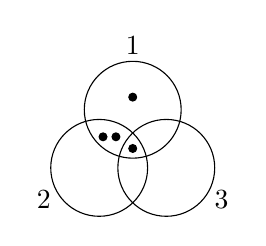
\begin{tikzpicture}]
    \tikzmath{
      \scale = 0.7;
      \rr = 2.5 * \scale;
      \aa = \scale;
      \bb = sqrt(3) * \aa;
      \cc = 2 * \aa;
      \topY = \cc + \rr;
      \crossLeftRightUpper = sqrt(\rr*\rr - \bb*\bb) - \aa;
      \dotTopY = ( \crossLeftRightUpper + \topY ) / 2;
      \dotTopLeftHeight = \crossLeftRightUpper - \scale/5;
      \dotTopLeftXFst = -\rr*0.48 - \scale/3;
      \dotTopLeftXSnd = -\rr*0.48 + \scale/3;
      \labelDist = \scale * 0.8;
      \labelTopY = \topY + \labelDist;
      \labelBottomX = \labelTopY * sqrt(3) / 2;
      \labelBottomY = \labelTopY / 2;
    }
    \draw (0, \cc em) circle [radius = \rr em];
    \draw (-\bb em, -\aa em) circle [radius = \rr em];
    \draw (+\bb em, -\aa em) circle [radius = \rr em];
    \node[draw,fill,shape=circle,scale=0.3] at (0,0) {};
    \node[draw,fill,shape=circle,scale=0.3] at (0, \dotTopY em) {};
    \node[draw,fill,shape=circle,scale=0.3]
    at (\dotTopLeftXFst em, \dotTopLeftHeight em) {};
    \node[draw,fill,shape=circle,scale=0.3]
    at (\dotTopLeftXSnd em, \dotTopLeftHeight em) {};
    \node at (0, \labelTopY em) {1};
    \node at (-\labelBottomX em, -\labelBottomY em) {2};
    \node at (+\labelBottomX em, -\labelBottomY em) {3};
  \end{tikzpicture},
  \label{eq:venn_diagram}
\end{align}
where $g_S$ is determined the number of dots at the intersection of
the circles $j\in S$.  We denote an assignment of distinct indices
according to choices of $g_S$ for all $S\in\PP\p{\ZZ_p}$ by $g$, where
$\PP\p{\ZZ_p}$ is the power set (i.e.~set of all subsets) of $\ZZ_p$.
Given a vector $\m M$ of the tensor ranks $M_j$, we then denote the
set of all valid index assignments $g$ by $\G\p{\m M}$.  For
consistency, all valid index assignments $g\in\G\p{\m M}$ must assign
exactly $M_j$ indices to the rank-$M_j$ tensor $w_j$, i.e.~
\begin{align}
  \sum_{S\in\PP\p{\ZZ_p}\,:\,j\in S} g_S
  = \sum_{R\in\PP\p{\ZZ_p\setminus\set{j}}} g_{\set{j}\cup R}
  = M_j
\end{align}
for all $j\in\ZZ_p$.  In order to make the index assignments
determined by choices of $g_S$ for all $S\in\PP\p{\ZZ_p}$ unique, we
also enforce that $g_{\set{}}=0$ for all $g\in\G\p{\m M}$, which is
equivalent to saying that every dot in the corresponding Venn diagram
must lie within some circle.  The set of valid index assignments
$\G\p{\m M}$ is then essentially the set of all Venn diagrams of the
form in \eqref{eq:venn_diagram} with $p=\rank\p{\m M}$ circles and a
total of $M_j$ dots within circle $j$.

A classification of terms in \eqref{eq:sym_prod_vec} by index
assignments $g\in\G\p{\m M}$ allows us to expand
\begin{align}
  \prod_{j\in\ZZ_p} \sum_{k\in\ZZ_N^{M_j}} w_j\p{k} O_j\p{k}
  \EQFS \sum_{g\in\G\p{\m M}} \S\p{g} w\p{g} O\p{g},
  \label{eq:sym_prod_group_start}
\end{align}
where $O\p{g}$ is an operator acquired by assigning indices to the
tensors $O_j$ in a manner consistent with $g$; $w\p{g}$ is a scalar
acquired by summing over all indices assigned to the tensors $w_j$
according to $g$; and $\S\p{g}$ is a symmetry factor accounting for
the number of equivalent ways to assign indices according to $g$.

In order to write out the factors in \eqref{eq:sym_prod_group_start}
explicitly, we identify the set of values that the distinct indices
assigned according to $g$ can take:
\begin{align}
  \C_N\p{g}
  \equiv \set{ k \in \bigotimes_{S\in\PP\p{\ZZ_p}} \C_N\p{g_S}
    : \t{all elements of $k$ are distinct} },
\end{align}
where each $k\in\C_N\p{g}$ has the natural decomposition
$k=\p{k_S:S\in\PP\p{\ZZ_p}}$ with $k_S\in\C_N\p{g_S}$.  We then define
the restriction of $k\in\C_N\p{g}$ to values associated with $w_j$ and
$O_j$:
\begin{align}
  k_j \equiv \bigcup_{S\in\PP\p{\ZZ_p} : j\in S} k_S
  = \bigcup_{R\in\PP\p{\ZZ_p\setminus\set{j}}} k_{\set{j}\cup R},
\end{align}
where the union of lists $k_S$ denotes a concatenation of those lists.
These definitions allow us to expand
\begin{align}
  w\p{g} \equiv \sum_{k\in\C_N\p{g}} \prod_{j\in\ZZ_p} w_j\p{k_j},
  &&
  O\p{g} \equiv \prod_{j\in\ZZ_p}
  O_j\p{\ell_j}~\t{for some}~\ell\in\C_N\p{g},
\end{align}
where the choice of $\ell\in\C_N\p{g}$ does not matter after
projection onto fully symmetric manifold, and
\begin{align}
  \S\p{g} \equiv \sp{\prod_{j\in\ZZ_p} { M_j \choose g_S : j\in S }}
  \sp{\prod_{S\in\PP\p{\ZZ_p}} \p{g_S!}^\abs{S}}
  = \prod_{j\in\ZZ_p} M_j!,
  \label{eq:sym_prod_symmetry}
\end{align}
where the first product in \eqref{eq:sym_prod_symmetry} contains
multinomial coefficients
\begin{align}
  { M \choose a_1, a_2, \cdots, a_m }
  \equiv \f{M!}{a_1!a_2!\cdots a_m!},
\end{align}
that account for the number of ways to partition the indices of each
$w_j,O_j$ into sets of shared indices according to $g_S$ for all
$j\in S$, and the second product in \eqref{eq:sym_prod_symmetry}
accounts for the number of ways to permute each set of shared indices
on every tensor.  Altogether, the symmetry factors $\S\p{g}$ cancel
out with the $\sim M_j!$ prefactors in \eqref{eq:sym_prod_vec}, so
\begin{align}
  \prod_{j\in\ZZ_p} \sum_{k\in\C_N\p{M_j}} w_j\p{k} O_j\p{k}
  \EQFS \sum_{g\in\G\p{\m M}} w\p{g} O\p{g}.
  \label{eq:sym_prod_group}
\end{align}

%%%%%%%%%%%%%%%%%%%%%%%%%%%%%%%%%%%%%%%%%%%%%%%%%%
\subsection{Single-body product}
\label{sec:PXYP}

Calculating the second-order effective Hamiltonian $H_1^{(2)}$ induced
on the fully symmetric manifold $\M_0$ by the perturbation $\V_1$ in
\eqref{eq:perturbations} requires us to simplify
\begin{align}
  \P_0 \p{\V_1^\Delta}^2 \P_0
  \EQFS \sum_{\substack{X,Y\\p,q}} v_{Xp} v_{Yq} X_p Y_q
  = \sum_{X,Y,p} v_{Xp} v_{Yp} X_p Y_p
  + \sum_{\substack{X,Y\\p\ne q}} v_{Xp} v_{Yq} X_p Y_q,
  \label{eq:PXYP_start}
\end{align}
where $\EQFS$ denotes equality under a restriction to the fully
symmetric manifold $\M_0$; and all coefficient vectors $\v v_X$
satisfy \eqref{eq:cond_1} with eigenvalue $\Delta\ne0$, which implies
that all $\v v_X$ are mean-zero.  The first sum on the right of
\eqref{eq:PXYP_start} is then
\begin{align}
  \sum_{X,Y,p} v_{Xp} v_{Yp} X_p Y_p
  \EQFS \sum_{X,Y,p} v_{Xp} v_{Yp} X_0 Y_0
  \EQFS \f1N \sum_{X,Y} \v v_X \c\v v_Y \col{XY},
  &&
  \col{Z} \equiv \sum_p Z_p.
  \label{eq:PXYP_eq}
\end{align}
The second sum on the right of \eqref{eq:PXYP_start}, meanwhile, is
\begin{align}
  \sum_{\substack{X,Y\\p\ne q}} v_{Xp} v_{Yq} X_p Y_q
  \EQFS \sum_{\substack{X,Y\\p\ne q}} v_{Xp} v_{Yq} X_0 Y_1,
  \label{eq:PXYP_neq_start}
\end{align}
where we can use the fact that the vectors $\v v_X,\v v_Y$ are
mean-zero to simplify the sum over $p\ne q$ in
\eqref{eq:PXYP_neq_start} to
\begin{align}
  \sum_{p\ne q} v_{Xp} v_{Yq}
  = \sum_{p,q} v_{Xp} v_{Yq} - \sum_{p=q} v_{Xp} v_{Yq}
  = - \v v_X\c\v v_Y,
\end{align}
In order to simplify the product of operators in
\eqref{eq:PXYP_neq_start}, we expand
\begin{align}
  \col{X}\,\col{Y} = \sum_{p,q} X_p Y_q
  = \sum_{p=q} X_p Y_q + \sum_{p\ne q} X_p Y_q
  \EQFS \col{XY} + N\p{N-1} X_0 Y_1,
  \label{eq:PXYP_neq_ops}
\end{align}
which implies that
\begin{align}
  \sum_{\substack{X,Y\\p\ne q}} v_{Xp} v_{Yq} X_p Y_q
  \EQFS - \sum_{X\ne Y} \v v_X\c\v v_Y X_0 Y_1
  \EQFS - \f1{N\p{N-1}}\sum_{X,Y} \v v_X\c\v v_Y
  \p{\col{X}\,\col{Y} - \col{XY}}.
  \label{eq:PXYP_neq}
\end{align}
Altogether, we have that
\begin{align}
  \P_0 \p{\V_1^\Delta}^2 \P_0
  = - \f1{N\p{N-1}} \sum_{X,Y} \v v_X \c\v v_Y
  \p{\col{X}\,\col{Y} - N \col{XY}}.
\end{align}

%%%%%%%%%%%%%%%%%%%%%%%%%%%%%%%%%%%%%%%%%%%%%%%%%%
\subsection{Two-body product}
\label{sec:POQP}

Calculating the second-order effective Hamiltonian $H_2^{(2)}$ induced
on the fully symmetric manifold $\M_0$ by the perturbation $\V_2$ in
\eqref{eq:perturbations} requires us to simplify
\begin{align}
  \P_0 \p{\V_2^\Delta}^2 \P_0
  = \sum_{O,Q} \sum_{\substack{k<\ell\\p<q}}
  w_{Ok\ell} w_{Qpq} O_{k\ell} Q_{pq}
  \EQFS \f14 \sum_{O,Q} \sum_{k,\ell,p,q}
  w_{Ok\ell} w_{Qpq} O_{k\ell} Q_{pq},
  \label{eq:POQP_start}
\end{align}
where $\EQFS$ denotes equality under a restriction to the fully
symmetric manifold $\M_0$; we define $w_{Opq}$ for all $p,q$ (as
opposed to only $p<q$) by enforcing $w_{Opq}=w_{Oqp}$ and $w_{Opp}=0$;
and the coefficient vectors $\v w_O$ satisfy the eigenvalue equation
\eqref{eq:cond_2} with eigenvalue $\Delta\ne0$, which implies that all
$\v{\m w}_O$ are mean-zero.  To simplify the sum in
\eqref{eq:POQP_start}, we first consider the terms with
$\p{p,q}=\p{k,\ell}$:
\begin{align}
  \sum_{k<\ell}
  w_{Ok\ell} w_{Qk\ell} O_{k\ell} Q_{k\ell}
  = \v{\m w}_O \c \v{\m w}_Q O_{1,2} Q_{1,2}.
\end{align}
We then consider terms $p\in\set{k,\ell}$ and $q\notin\set{k,\ell}$ or
vice versa:
\begin{align}
  \f14 \sum_{\substack{k,\ell\\p\in\set{k,\ell}\\q\notin\set{k,\ell}}}
  w_{Ok\ell} w_{Qpq} O_{k\ell} Q_{pq}
  &\EQFS \f12 \sum_{\substack{k,\ell\\q\notin\set{k,\ell}}}
  w_{Ok\ell} w_{Qkq} O_{1,2} Q_{2,3} \\
  \f14 \sum_{\substack{k,\ell\\p\notin\set{k,\ell}\\q\in\set{k,\ell}}}
  w_{Ok\ell} w_{Qpq} O_{k\ell} Q_{pq}
  &\EQFS \f12 \sum_{\substack{k,\ell\\q\notin\set{k,\ell}}}
  w_{Ok\ell} w_{Qkq} O_{1,2} Q_{2,3},
\end{align}
where
\begin{align}
  \sum_{\substack{k,\ell\\q\notin\set{k,\ell}}} w_{Ok\ell} w_{Qkq}
  = \sum_{k,\ell,q} w_{Ok\ell} w_{Qkq}
  - \sum_{k,\ell} w_{Ok\ell} w_{Qk\ell}
  = \v w_O\c\v w_Q - 2 \v{\m w}_O \c \v{\m w}_Q.
\end{align}
Finally, the terms in \eqref{eq:POQP_start} with
$p,q\notin\set{k,\ell}$ are
\begin{align}
  \f14 \sum_{\substack{k,\ell\\p,q\notin\set{k,\ell}}}
  w_{Ok\ell} w_{Qpq} O_{k\ell} Q_{pq}
  \EQFS \f14 \sum_{\substack{k,\ell\\p,q\notin\set{k,\ell}}}
  w_{Ok\ell} w_{Qpq} O_{1,2} Q_{3,4},
\end{align}
where, using the fact that all $\v{\m w}_O$ are mean-zero,
\begin{multline}
  \f14 \sum_{\substack{k,\ell\\p,q\notin\set{k,\ell}}} w_{Ok\ell} w_{Qpq}
  = - \f14 \sum_{\substack{k,\ell\\p,q\in\set{k,\ell}}} w_{Ok\ell} w_{Qpq}
  - \f14 \sum_{\substack{k,\ell\\p\in\set{k,\ell}\\q\notin\set{k,\ell}}}
  w_{Ok\ell} w_{Qpq}
  - \f14 \sum_{\substack{k,\ell\\p\notin\set{k,\ell}\\q\in\set{k,\ell}}}
  w_{Ok\ell} w_{Qpq} \\
  = -\v w_O \c \v w_Q + \v{\m w}_O \c \v{\m w}_Q.
\end{multline}
Altogether, we thus have that
\begin{multline}
  \P_0 \p{\V_2^\Delta}^2 \P_0
  \EQFS \sum_{O,Q}
  \bigg[ \v{\m w}_O \c \v{\m w}_Q O_{1,2} Q_{1,2}
  + \p{\v w_O\c\v w_Q - 2 \v{\m w}_O \c \v{\m w}_Q}
  O_{1,2} Q_{2,3} \\
    - \p{\v w_O \c \v w_Q - \v{\m w}_O \c \v{\m w}_Q}
    O_{1,2} Q_{3,4} \bigg].
  \label{eq:POQP}
\end{multline}
In principle, our next task is to write this result in terms of
collective operators within the fully symmetric manifold; this task
turns out to be rather non-trivial in general.  We therefore discuss
the decomposition of multi-local operators (e.g.~$O_{1,2} Q_{2,3}$, a
3-local operator) into a sum of collective operators within the fully
symmetric manifold in Appendix \ref{sec:multi_to_collective}.  At the
end of Appendix \ref{sec:multi_to_collective}, we provide analytical
expressions for the special cases of
\begin{enumerate*}
\item multi-local operators that are tensor powers of a single
  operator, i.e.~of the form $X^{\otimes k}$; and
\item multi-local operators of the form $X^{\otimes k}$ with $X^2=1$.
\end{enumerate*}
These cases are relevant for e.g.~the SU(2) case with Ising-type
interactions of the form $Z\otimes Z$, with $Z$ a single-spin Pauli
operator.

%%%%%%%%%%%%%%%%%%%%%%%%%%%%%%%%%%%%%%%%%%%%%%%%%%%%%%%%%%%%%%%%%%%%%%
\section{Analytical results in translationally invariant systems}
\label{sec:trans_inv}

Here we simplify the eigenvalue problems that appear at second order
in the single- and two-body theory in Sections
\ref{sec:single_body_pert} and \ref{sec:two_body_pert} in the case of
a translationally invariant system with periodic boundary conditions.
We solve the single-body eigenvalue problem analytically, and reduce
the two-body eigenvalue problem to that of diagonalizing
$\p{N-1}\times\p{N-1}$ matrices.  Finally, for we discuss the further
reduction of the two-body problem to that of diagonalizing matrices
with dimensions $\sim\p{N/2^D}\times\p{N/2^D}$ in the case of an
isotropic system on a $D$-dimensional periodic lattice, but leave this
reduction to future work.

%%%%%%%%%%%%%%%%%%%%%%%%%%%%%%%%%%%%%%%%%%%%%%%%%%
\subsection{Single-body eigenvalue problem}
\label{sec:trans_inv_single}

For reference, the single-body eigenvalue problem is
\begin{align}
  \p{\m h - \diag\v h}\c\v v = \Delta \v v,
  \label{eq:cond_1_ref}
\end{align}
where $\m h$ is a matrix of all couplings $h_{pq}$ that appear in the
interaction Hamiltonian $H_0$ in \eqref{eq:ints}; $\v h$ is a vector
of all $h_p\equiv\sum_q h_{pq}$; $\diag\v h$ is a matrix with $\v h$
on the diagonal and zeroes everywhere else; and $\v v$ is a vector of
coefficients used to construct the single-body perturbation
$\V_1\p{\v v}$ defined in \eqref{eq:perturbations}.  When the
interaction Hamiltonian $H_0$ is translationally invariant, the
couplings $h_{pq}$ depend only on the separation $\pm\p{p-q}$, so the
eigenvectors of $\m h$ are plane waves of the form
\begin{align}
  \v v_k \equiv \sum_p e^{ip\c k} \ket{p},
\end{align}
where on a $D$-dimensional periodic lattice of $N=L^D$ spins, lattice
sites are indexed by vectors
$p\in\ZZ_L^D\simeq\set{0,1,\cdots,L-1}^{\otimes D}$, and wavenumbers
take on values $k\in\ZZ_L^D\times2\pi/L$.  The corresponding
eigenvalues of $\m h$ can be determined by expanding
\begin{align}
  \m h\c\v v_k = \sum_{p,q} h_{pq} e^{iq\c k} \ket{p}
  = \sum_{p,d} h_{p,p+d} e^{i\p{p+d}\c k} \ket{p}
  = \sum_d h_{0,d} e^{id\c k} \v v_k
  = \sum_d h_{0,d} \cos\p{d\c k} \v v_k,
\end{align}
where the imaginary terms vanish because $h_{0,d}=h_{0,-d}$.  The
remainder of \eqref{eq:cond_1_ref} that we need to sort out is
$\diag\v h$, where all $h_p=\sum_qh_{pq}=\sum_dh_{0,d}$ are equal,
which implies that $\diag\v h=\sum_dh_{0,d}$ is a scalar.  We thus
find that
\begin{align}
  \p{\m h - \diag\v h}\c\v v_k = \Delta_k \v v_k,
  &&
  \Delta_k \equiv \sum_d h_{0,d} \sp{\cos\p{d\c k}-1}.
\end{align}

%%%%%%%%%%%%%%%%%%%%%%%%%%%%%%%%%%%%%%%%%%%%%%%%%%
\subsection{Two-body eigenvalue problem}
\label{sec:trans_inv_two}

The two-body eigenvalue equation in \eqref{eq:cond_2} is designed to
find solutions $\m w$ to the equation
\begin{align}
  \bar h_{pq} w_{pq}
  + \sum_k \p{h_{pk} w_{kq} + w_{pk} h_{kq}}
  = \Delta w_{pq},
  &&
  \bar h_{pq} \equiv 2h_{pq} - h_p - h_q,
  &&
  h_p \equiv \sum_q h_{pq},
  \label{eq:cond_2_ref_start}
\end{align}
which can be written in matrix form as
\begin{align}
  \bar{\m h} * \m w + \P_{\t{off-diag}}\p{\m h\c\m w + \m w\c\m h}
  = \Delta \m w,
  \label{eq:cond_2_ref}
\end{align}
where $\m h$, $\bar{\m h}$, and $\m w$ are matrices of all $h_{pq}$,
$\bar h_{pq}$ and $w_{pq}$; $\bar{\m h}*\m w$ denotes an element-wise
(Kronecker) product of $\bar{\m h}$ and $\m w$, i.e.~with matrix
elements $\bar h_{pq}w_{pq}$; and
$\P_{\t{off-diag}}\p{\m m}\equiv \m m-\sum_p\op{p}\m m\op{p}$ denotes
the projection of $\m m$ onto the space of strictly off-diagonal
matrices.  In order to find solutions to \eqref{eq:cond_2_ref} when
the interaction Hamiltonian $H_0$ is translationally invariant, in
which case $h_{pq}$ and $\bar h_{pq}$ depend only on the separation
$\pm\p{p-q}$, we expand all matrices in a basis that the respects
translational symmetry.  To this end, for all lattice displacements
$d\in\ZZ_L^D$ and wavenumbers $k\in\ZZ_L^D\times2\pi/L$ we define the
{\it cycle matrices}
\begin{align}
  \m m_{dk} \equiv \sum_p e^{ip\c k} \op{p+d}{p},
  \label{eq:cycle}
\end{align}
where the element-wise sums in $p+d$ are implicitly taken modulo $L$
(i.e.~the length of the periodic lattice along each axis).  In terms
of these cycle matrices, we define
\begin{align}
  \tilde w_{dk} \equiv \f1N \tr\p{\m m_{dk}^\dag \m w},
\end{align}
and expand
\begin{align}
  \m w = \sum_{d,k} \tilde w_{dk} \m m_{dk},
  &&
  \m h = \sum_{q,d} h_{q+d,q} \op{q+d}{q}
  = \sum_d h_{d,0} \m m_{d,0},
  &&
  \bar{\m h} = \sum_d \bar h_{d,0} \m m_{d,0}.
\end{align}
We can then write the condition in \eqref{eq:cond_2_ref} as a new set
of conditions
\begin{align}
  \sum_{d\ne0} \bar h_{d,0} \tilde w_{dk} \m m_{dk}
  + \sum_{\substack{c,d\\c+d\ne0}}
  h_{c,0} \tilde w_{dk} \p{1 + e^{-ic\c k}} \m m_{c+d,k}
  = \Delta \sum_{d\ne0} \tilde w_{dk} \m m_{dk},
\end{align}
that must hold for all wavenumbers $k$.  With some re-indexing, we can
write
\begin{align}
  \sum_{d\ne0} \bar h_{d,0} \tilde w_{dk} \m m_{dk}
  + \sum_{c,d\ne0} h_{d-c,0} \tilde w_{ck}
  \p{1 + e^{-i\p{d-c}\c k}} \m m_{dk}
  = \Delta \sum_{d\ne0} \tilde w_{dk} \m m_{dk},
  \label{eq:cond_2_cycle}
\end{align}
and define
\begin{align}
  \ut{\check{\m h}}_k
  \equiv \sum_{d\ne0} \bar h_{d,0} \op{d}
  + \sum_{c,d\ne0} h_{d-c,0} \p{1+e^{-i\p{d-c}\c k}} \op{d}{c},
  &&
  \ut{\v{\m w}}_k \equiv \sum_{d\ne0} \tilde w_{dk} \ket{d},
  \label{eq:cycle_vecs}
\end{align}
in order to express \eqref{eq:cond_2_cycle} as the set of eigenvalue
equations
\begin{align}
  \ut{\check{\m h}}_k \c \ut{\v{\m w}}_k = \Delta \ut{\v{\m w}}_k.
  \label{eq:cond_2_square}
\end{align}
The appearance of a wavenumber index $k$ in \eqref{eq:cond_2_square}
implies that all fixed-$k$ components of a general coefficient matrix
$\m w$ must simultaneously satisfy \eqref{eq:cond_2_square} in order
to generate states of fixed excitation energy $\Delta$ when the
corresponding perturbation $\V_2^\Delta$ acts on a fully symmetric
state $\ket\psi\in\M_0$.  The decomposition of an arbitrary
coefficient vector $\v{\m w}=\sum_\Delta\v{\m w}_\Delta$ into
coefficient vectors $\v{\m w}_\Delta$ that generate a fixed-energy
perturbation $\V_2^\Delta$ is then performed by projecting each
$k$-component of $\v{\m w}$ onto the corresponding $\Delta$-eigenspace
of $\ut{\check{\m h}}_k$.  If the perturbation $\V_2$ is
translationally invariant, then the $k$-components of $\v{\m w}$ for
all $k\ne 0$ all vanish, so we only need to consider the case of
$k=0$.

We can reduce the eigenvalue problem in \eqref{eq:cond_2_square} even
further in the case of an isotropic system, in which the couplings
$h_{pq}$ depend only on the distance $\abs{p-q}$.  On a $D$
dimensional lattice, isotropy implies one reflection symmetry for each
lattice axis, which reduces the degrees of freedom in of
$\ut{\check{\m h}}_k$ from $\sim N\times N$ to
$\sim\p{N/2^D}\times\p{N/2^D}$.  We leave this reduction to future
work.

%%%%%%%%%%%%%%%%%%%%%%%%%%%%%%%%%%%%%%%%%%%%%%%%%%
\subsection{The fully collective model}

Here we solve the single- and two-body eigenvalue problems in the case
of a fully collective spin model with uniform couplings:
$h_{pq}=-1+\delta_{pq}$.  In this case, the single-body excitation
energies $\Delta_k$ are
\begin{align}
  \Delta_k
  = - \sum_{d\ne 0} \sp{\cos\p{d\c k}-1}
  = N \p{1-\delta_{k,0}}.
\end{align}
In order to solve the two-body eigenvalue problem, we expand
\begin{align}
  \ut{\check{\m h}}_k
  &= \sum_{d\ne0} \sp{-2+2\p{N-1}} \op{d}
  - \sum_{\substack{c,d\ne0\\c\ne d}} \p{1+e^{-i\p{d-c}\c k}} \op{d}{c} \\
  &= 2\p{N-1} \1_{N-1}
  - \sum_{c,d\ne0} \p{1+e^{-i\p{d-c}\c k}} \op{d}{c},
\end{align}
where $\1_{N-1}\equiv\sum_{d\ne0}\op{d}$ is the $\p{N-1}\times\p{N-1}$
identity matrix, and define the vectors
\begin{align}
  \ket{\ut{p}}
  \equiv \f1{\sqrt{N-1}} \sum_{d\ne 0} e^{i p\c d}\ket{d},
\end{align}
in terms of which
\begin{align}
  \ut{\check{\m h}}_k
  = 2\p{N-1} \1_{N-1} -\p{N-1} \p{\op{\ut{0}} + \op{\ut{k}}}.
\end{align}
The vectors $\ket{\ut{p}}$ are normalized, but not orthogonal:
$\braket{\ut{p}|\ut{q}}=\delta_{pq}-\p{1-\delta_{pq}}/\p{N-1}$.  We
therefore have
\begin{align}
  \ut{\check{\m h}}_k
  = 2\p{N-1} \1_{N-1} - \sum_{s\in\set{\pm}} \varepsilon_s \op{\ut{k}^s}
\end{align}
where
\begin{align}
  \varepsilon_\pm \equiv N - 1 \mp 1,
  &&
  \ket{\ut{k}^\pm}
  \equiv \p{1\mp\f1{N-1}}^{-1/2}
  \f{\ket{\ut{0}}\pm\ket{\ut{k}}}{\sqrt{2}}.
\end{align}
The vectors $\ket{\ut{k}^\pm}$ are orthonormal when $k\ne0$.  When
$k=0$, meanwhile, we have
\begin{align}
  \ut{\check{\m h}}_0 = 2\p{N-1} \p{\1_{N-1} - \op{\ut{0}}}.
\end{align}
Remembering from \eqref{eq:cycle_vecs} that vectors $\ket{\ut{k}^\pm}$
are associated with the cycle matrices $\m m_{dk}$ defined in
\eqref{eq:cycle} via
\begin{align}
  \ket{\ut{k}^\pm}
  \propto \ket{\ut{0}} \pm \ket{\ut{k}}
  \propto \sum_{d\ne0} \p{1 \pm e^{ik\c d}} \ket{d}
  \to \sum_{d\ne0} \p{1 \pm e^{ik\c d}} \m m_{dk},
\end{align}
one can work out that the vectors $\ket{\ut{k}^\pm}$ correspond to
matrices that are strictly symmetric ($+$) or anti-symmetric ($-$)
under transposition.  The two-body perturbations considered in this
work, however, are defined using coefficient vectors
$\set{\v{\m w}_O}$ that correspond to symmetric matrices
$\set{\m w_O}$, with $w_{Opq}=w_{Oqp}$.  We can therefore neglect the
eigenvectors $\ket{\ut{k}^-}$ and corresponding eigenvalues
$\varepsilon_-$ entirely for the purposes of this work.

Altogether, the excitation energies corresponding to non-trivial
eigenstates of $\ut{\check{\m h}}_k$ are
\begin{align}
  \Delta_0 \equiv 0,
  &&
  \Delta_+ \equiv 2\p{N-1} - \varepsilon_+ = N,
\end{align}
while the energy of all orthogonal two-body excitations is
\begin{align}
  \Delta_\perp \equiv 2\p{N-1}.
\end{align}

%%%%%%%%%%%%%%%%%%%%%%%%%%%%%%%%%%%%%%%%%%%%%%%%%%%%%%%%%%%%%%%%%%%%%%
\section{Collective and multi-local operators in the fully symmetric
  manifold}
\label{sec:multi_to_collective}

Here we provide a decomposition multi-local operators into sums of
collective operators (and vice versa) within the fully symmetric
manifold of $N$ spins.  Multi-local operators are operators of the
form
\begin{align}
  O_S \equiv \bigotimes_{O\in S} O,
  \label{eq:multi_op_set}
\end{align}
where $S\equiv\set{O}$ is a set of single-spin operators $O$.  The
order of tensor factors in \eqref{eq:multi_op_set} does not matter
after projecting operators onto the fully symmetric manifold, as we
always will in this section.  While the decomposition of a collective
operator into a sum of multi-local operators is unique, the opposite
is not true: there is generally no unique decomposition of a
multi-local operator into a sum of collective operators.  We can,
however, enforce a canonical decomposition by choosing a set of
collective operators that obey the same symmetries as $O_S$, namely
invariance under arbitrary permutations of the single-spin operators
$O\in S$.

Even though $S$ contains $\abs{S}$ spins, a collective operator built
from the single-spin operators $O\in S$ may have multiple
(single-spin) operators acting on the same spin, resulting in a
$k$-local operator with $k<\abs{S}$.  We therefore {\it
  partition}\footnote{A partition $P\equiv\set{p}$ of $S$ is a set of
  mutually disjoint, non-empty subsets $p\subset S$ with
  $\bigcup_{p\in P}p=S$.} $S$ into subsets of operators that act on
the same spin.  For any partition $P\equiv\set{p}$ of $S$ (here
$p\subset S$ is a subset of operators $O\in S$ that address the same
spin), we then define the $\abs{P}$-local operator
\begin{align}
  O_P \equiv \bigotimes_{p\in P} \bigodot_{O\in p} O,
\end{align}
where $\bigodot_{x\in\X} x$ denotes a symmetrized product of all
elements in $\X$, i.e.
\begin{align}
  \bigodot_{x\in\X} x
  \equiv \f1{\abs{\X}!}
  \sum_{\substack{\t{permutations}\\\sigma~\t{of}~\X}}
  ~ \prod_{k=1}^{\abs{\X}} x_{\sigma_k},
\end{align}
with $\sigma_k$ the $k$-th element of the permutation $\sigma$ when
expressed in one-line notation; for example,
\begin{align}
  \bigodot_{j=1}^2 x_j &= x_1 \odot x_2 = \f12 \p{x_1x_2 + x_2x_1}, \\
  \bigodot_{j=1}^3 x_j
  &= \f1{3!} \p{x_1x_2x_3 + x_1x_3x_2 + x_2x_1x_3
    + x_2x_3x_1 + x_3x_1x_2 + x_3x_2x_1}.
\end{align}
The set of multi-local operators $\set{O_P:\t{partitions}~P~\t{of}~S}$
consists of all operators that
\begin{enumerate*}
\item can be built from ordinary products and tensor products of all
  single-spin operators $O\in S$, and
\item are invariant under arbitrary permutations of $S$.
\end{enumerate*}
For any set $S$ of single-spin operators and any partition $P$ of $S$,
we can similarly define the collective operators
\begin{align}
  \O_S \equiv \bigodot_{O\in S} \col{O},
  &&
  \O_P \equiv \bigodot_{p\in P} \col{\textstyle\bigodot_{O\in p} O},
\end{align}
where we underline a single-spin operator to denote its collective
version, i.e.~$\col{Q}\equiv\sum_j Q^{(j)}$, where $Q^{(j)}$ is an
operator that acts with the single-spin operator $Q$ on spin $j$ and
trivially on all other spins.  By construction, the set of collective
operators $\set{\O_P:\t{partitions}~P~\t{of}~S}$ is one-to-one to the
set of multi-local operators $\set{O_P:\t{partitions}~P~\t{of}~S}$,
and it is straightforward to work out that for any set $S$ of
single-spin operators,
\begin{align}
  \O_S
  \EQFS \sum_{\substack{\t{partitions}\\P~\t{of}~S}}
  N!_{\abs{P}} O_P,
  &&
  N!_k \equiv \prod_{j=0}^{k-1}\p{N-j}! = \f{N!}{\p{N-k}!},
  \label{eq:collective_to_multi_full}
\end{align}
where $\EQFS$ denotes equality under a restriction to the fully
symmetric manifold.  For any multi-local operator $O_S$ indexed by a
set $S$ of single-spin operators, we can collect expansions of the
form \eqref{eq:collective_to_multi_full} for all collective operators
built from non-empty subsets of $S$ into a system of linear equations
$\L$, and in turn solve $\L$ for $O_S$.  When
$\abs{S}\in\set{1,2,3,4}$ (and, by conjecture, for all $S$), by use of
a computer algebra system (namely, Mathematica) we find that
\begin{align}
  N!_{\abs{S}} O_S
  &\EQFS \sum_{\substack{\t{partitions}\\P~\t{of}~S}}
  \p{-1}^{\abs{S}-\abs{P}} \O_P \times \prod_{p\in P}\p{\abs{p}-1}!
  \label{eq:multi_to_collective_full} \\
  &\EQFS \f1{\abs{S}!} \sum_{\substack{\t{permutations}\\\Pi~\t{of}~S}}
  \sum_{\substack{\t{ordered}\\\t{partitions}\\\tilde P~\t{of}~\Pi}}
  \p{-1}^{\abs{S}-\abs{\tilde P}} \O_{\tilde P}
  \times \prod_{\tilde p\in\tilde P} \p{\abs{\tilde p}-1}!
  \label{eq:multi_to_collective_full_simp}
\end{align}
where we identify permutations $\Pi$ of $S$ with an ordered list
(tuple) $\p{O_1,O_2,\cdots,O_{\abs{S}}}$ of all single-spin operators
in $S$; and we enforce that partitions $\tilde P$ of an ordered list
$\Pi$, as well as parts $\tilde p\in\tilde P$, are lexicographically
ordered in accordance with the ordering of operators in $\Pi$.  If
$S=\set{X,Y,Z}$, for example, then the ordered partitions of the
trivial permutation $\Pi=\p{X,Y,Z}$ are
\begin{align}
  \p{\p{X,Y,Z}}, &&
  \p{\p{X,Y},\p{Z}}, &&
  \p{\p{X,Z},\p{Y}}, &&
  \p{\p{X},\p{Y,Z}}, &&
  \p{\p{X},\p{Y},\p{Z}}.
\end{align}
For ordered lists $\tilde S$ and ordered partitions $\tilde P$, we
define
\begin{align}
  O_{\tilde S} \equiv \bigotimes_{O\in\tilde S} O,
  &&
  O_{\tilde P}
  \equiv \bigotimes_{\tilde p\in\tilde P} \prod_{O\in\tilde p} O,
  &&
  \O_{\tilde S} \equiv \prod_{O\in\tilde S} \col{O},
  &&
  \O_{\tilde P}
  \equiv \prod_{\tilde p\in\tilde P}
  \col{\textstyle\prod_{O\in\tilde p} O},
\end{align}
where products over elements of $\tilde S,\tilde P,\tilde p$ are taken
in order according to the elements of these ordered lists, e.g.~if
$\tilde S=\p{O_1,O_2,\cdots,O_{\abs{S}}}$, then
$\prod_{O\in\tilde S}\equiv O_1O_2\cdots O_{\abs{S}}$.  These
definitions allow us to expand
\begin{align}
  \O_{\tilde S} \EQFS
  \sum_{\substack{\t{ordered}\\\t{partitions}\\\tilde P~\t{of}~\tilde S}}
  N!_{\abs{\tilde P}} O_{\tilde P},
\end{align}
in analogy to \eqref{eq:collective_to_multi_full}.

While the expansions in \eqref{eq:multi_to_collective_full} and
\eqref{eq:multi_to_collective_full_simp} closely resemble each other,
in practice the latter involves less computational overhead due to the
lack of symmetrization in the construction of $\O_{\tilde P}$.  There
are, in principle, even more economical decompositions of a
multi-local operators into collective opreators, for example
\begin{align}
  N!_2 X\otimes Y
  &\EQFS \col{X}\,\col{Y} - \col{XY}, \\
  N!_3 X\otimes Y \otimes Z
  &\EQFS \col{X}\,\col{Y}\,\col{Z}
  - \col{X}\,\col{YZ} - \col{Y}\,\col{XZ} - \col{Z}\,\col{XY}
  + \col{ZXY} + \col{YXZ},
\end{align}
but these decompositions generally do not preserve the manifest
symmetry of a multi-local operator $O_S$ under arbitrary permutations
of $S$, and we do not know of any general prescription to arrive at
such decompositions aside from solving systems of equations relating
collective operators to multi-local operators.

On a final note, we consider the special case that all operators
$O\in S$ are identical, for which we provide the expansions
\begin{align}
  N!_2 X\otimes X \EQFS \col{X}^2 - \col{X^2},
  &&
  N!_3 X^{\otimes 3} \EQFS \col{X}^3
  - 3 \col{X} \odot \col{X^2} + 2\col{X^3},
\end{align}
\begin{align}
  N!_4 X^{\otimes 4}
  \EQFS \col{X}^4 - 4 \col{X}^2 \odot \col{X^2}
  - 2 \col{X} \, \col{X}^2 \, \col{X}
  + 3 \p{\col{X^2}}^2 + 8 \col{X} \odot \col{X^3}
  - 6 \col{X^4}.
\end{align}
If furthermore $X^2=1$, as with e.g.~the Pauli operators of SU(2),
then
\begin{align}
  N!_2 X\otimes X \EQFS \col{X}^2 - N,
  &&
  N!_3 X^{\otimes 3} \EQFS \col{X}^3 - \p{3N-2} \col{X},
\end{align}
\begin{align}
  N!_4 X^{\otimes 4} \EQFS \col{X}^4
  - 2\p{3N-4} \col{X}^2 + 3 N \p{N-2}.
\end{align}

\bibliography{multilevel_spin_notes.bib}

\end{document}
